
\begin{questions}
\question{
Analytical solution of the model
}
\begin{solution}
  In this case we need to solve the Schrödinger equation

  \begin{equation}
    \left(-\frac{\hbar^2}{2m}\frac{d^2}{dx^2} + V(x)\right)\phi_{nk}(x) = E_{nk}\phi_{nk}(x).
  \end{equation}

  If $V(x)$ is a periodic potential we know we don't have to solve the problem for all space, since Bloch theorem tells us that the solutions will be the product of plane waves and a periodic function. Assuming that $V_1<E<V_2$ we will have

  \begin{equation}
    \phi_{nk}(x) = \begin{cases}
      Ae^{iKx} + Be^{-iKx}, \quad 0<x<b,\\
      Ce^{Qx} + De^{-Qx}, \quad -a < x < 0.
  \end{cases}
  \end{equation}
  With
  \begin{eqnarray}
    K = \sqrt{\frac{2m(E-V_1)}{\hbar^2}},\\
    Q = \sqrt{\frac{2m(V_2-E)}{\hbar^2}}.
  \end{eqnarray}
  By Bloch theorem, we know that
  \begin{equation}
    \phi_{nk}(b<x<b+a) = \phi_{nk}(-a<x<0)e^{ik(b+a)}.
    \label{bloch}
  \end{equation}
  Moreover, we know that the solution must be continuous, this imposes boundary conditions at $x=0$, and $x=b$.
  When $x=0$ both solutions will look like this
  \begin{eqnarray}
    A+B = C+D\\
    iK(A-B) = Q(C-D)
  \end{eqnarray}
  At $x=b$, using the condition in eq. \ref{bloch} we will have $\phi(-a)e^{ik(b+a)} = \phi(b)$, and a condition for the derivatives $\phi'(-a)e^{ik(b+a)}=\phi'(b)$ we have
  \begin{eqnarray}
    Ae^{iKb} + Be^{-iKb} = \left(Ce^{-Qa} + De^{Qa}\right)e^{ik(b+a)}\\
    iK\left(Ae^{iKb} + Be^{-iKb}\right) = Q\left(Ce^{-Qa} - De^{Qa}\right)e^{ik(b+a)}
  \end{eqnarray}
  Solving this four equation simultaneously leads us to ask for this determinant to be zero
  \begin{equation}
    \begin{vmatrix}
      1&1&-1&-1\\
      iK&-iK&-Q&Q\\
      e^{iKb}&e^{-iKb}&-e^{-Qa}e^{ik(b+a)}&-e^{Qa}e^{ik(b+a)}\\
      iKe^{iKb}&-iKe^{-iKb}&-Qe^{-Qa}e^{ik(b+a)}&Qe^{Qa}e^{ik(b+a)}
    \end{vmatrix} = 0.
  \end{equation}
  When we solve this determinant (by Mathematica) we get the following result
  \begin{equation}
    \left(\frac{Q^2 - K^2}{2QK}\right)\sinh(Qa)\sin(Kb) + \cosh(Qa)\cos(Kb) = cos(k(b+a)).
    \label{eq:num}
  \end{equation}
  We can introduce extra simplifications by taking the limit $b\rightarrow0$ and $V_2\rightarrow \infty$. While keeping $Q^2ba/2 = P$ constant. This means particularly that $Q\gg K$, and $Qa\ll 1$. So, we will have
  \begin{equation}
    f(Kb) = \frac{P}{Kb}\sin(Kb) + \cos(Kb) = \cos(kb).
    \label{alm}
  \end{equation}
  Here we can see clearly that the only allowed solutions are the ones with $-1\leq f(Kb)\leq1$

 Not all arguments fulfill this condition, as we can see in fig. \ref{sample}

 \begin{center}
   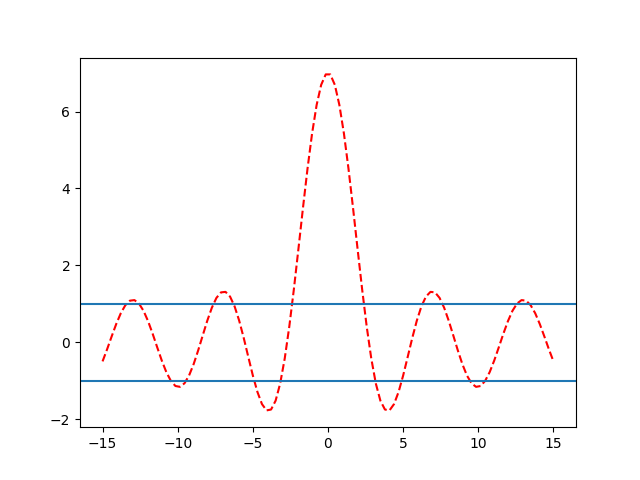
\includegraphics[width=85mm]{sample}
 \end{center}

 \captionof{figure}{Plot of the qualitative behavior of eq. \ref{alm}.}\label{sample}\vspace{0.5cm}


If we solve eq. \ref{eq:num} numerically we will find the band structure displayed in fig. \ref{num}

 \begin{center}
   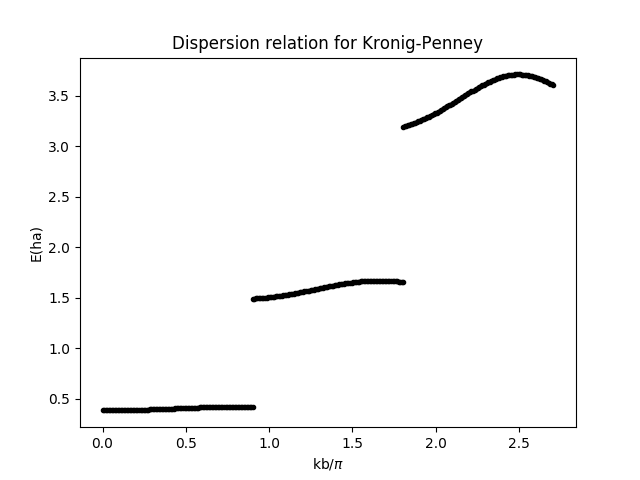
\includegraphics[width=99mm]{numsol}
 \end{center}

 \captionof{figure}{Band structure of the given material.}\label{num}\vspace{0.5cm}

Finally we can have an idea of the density of states just by counting and displaying the histogram showed in fig. \ref{hist}

\begin{center}
  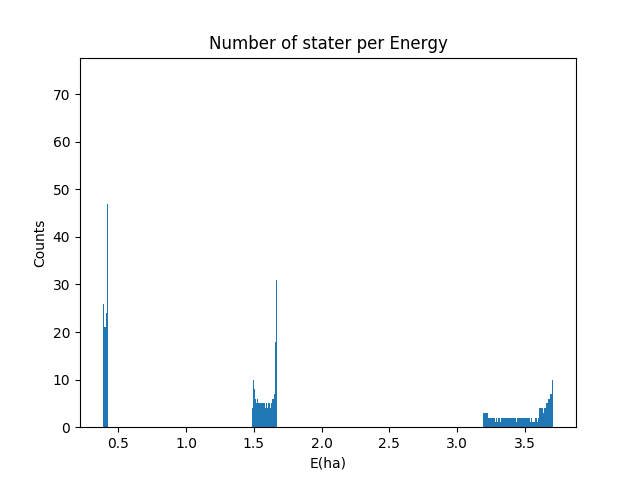
\includegraphics[width=85mm]{hist}
\end{center}

\captionof{figure}{Number of solutions for k as function of E.}\label{hist}\vspace{0.5cm}

Here we can see that we have more states close to the gaps that in the middle section of the bands.\\

 But I'm missing the Fermi energy, the reason is the following. In the model of Kronig-Penney there is no statement concerning the position of the Fermi level, for more information read \url{https://www.springer.com/cda/content/document/cda_downloaddocument/9783319197630-c2.pdf?SGWID=0-0-45-1514427-p177405762}

 I do not add the codes because it does not add anything new to the analysis, but they can be found here \url{https://github.com/UriAceves/QuantumTheoryofMaterialsHW/tree/master/HW06}

 \end{solution}

\end{questions}

%
% \begin{center}
%   \includegraphics[width=55mm]{}
% \end{center}
%
% \captionof{figure}{}\label{new}\vspace{0.5cm}
